\documentclass{homework}

\definecolor{bg}{rgb}{0.95,0.95,0.95}

\begin{document}
\frontpage{Þýðendur}{Compiler-NanoMorpho}{Guðmundur Óli Norland}{Egill Ragnarsson}{Snorri Agnarsson}

\begin{question}{Upplýsingar}
\end{question}
\begin{answer}
  \href{https://github.com/slowpokesheep/thydendur/tree/master/nanomorpho/nanomorpho}{Github}
  \begin{description}
    \item[NanoMorphoCompiler] - Er milliþulusmiður og lokaþulusmiður
    \item[NanoMorphoLexer] - Er lesgreinir ásamt \textbf{nanomorpho.flex}
  \end{description}
  Neðst má sjá að compiler'inn okkar breytt skránni \textbf{test.nm} í morpho assembler kóða, \textbf{test.masm} og svo loks keyrslu á þeirri skrá.
\end{answer}

\begin{question}{NanoMorphoCompiler}
\end{question}
\begin{answer}
  \begin{minted}[autogobble,tabsize=2, bgcolor=bg,breaklines,breakanywhere]{java}
  package nanomorpho;

import java.io.PrintWriter;
import java.util.Vector;
import java.util.HashMap;

public class NanoMorphoCompiler {

  static final int ERROR   = NanoMorphoLexer.ERROR;
  static final int IF      = NanoMorphoLexer.IF;
  static final int ELSE    = NanoMorphoLexer.ELSE;
  static final int ELSIF   = NanoMorphoLexer.ELSIF;
  static final int WHILE   = NanoMorphoLexer.WHILE;
  static final int VAR     = NanoMorphoLexer.VAR;
  static final int RETURN  = NanoMorphoLexer.RETURN;
  static final int NAME    = NanoMorphoLexer.NAME;
  static final int OPNAME  = NanoMorphoLexer.OPNAME;
  static final int LITERAL = NanoMorphoLexer.LITERAL;

  static PrintWriter writer;

  // Intermediate code element identification strings
  enum type {
    RETURN, STORE, OR, AND, NOT, CALL, FETCH, LITERAL, IF, WHILE, BODY
  }

  // Expressions:
  // ["RETURN",expr]
  // ["STORE",pos,expr]
  // ["OR",expr,expr]
  // ["AND",expr,expr]
  // ["NOT",expr]
  // ["CALL",name,args]
  // ["FETCH",pos]
  // ["LITERAL",string]
  // ["IF",expr,expr,expr]
  // ["WHILE",expr,expr]
  // ["BODY",exprs]

  // Forward one lexeme.
  // Returns the lexeme advanced over.
  static String advance() throws Exception {
    return NanoMorphoLexer.advance();
  }

  // Forward one lexeme which must have the given token.
  // Returns the lexeme advanced over.
  static String over(int token) throws Exception {
    return NanoMorphoLexer.over(token);
  }
  static String over(char token) throws Exception {
    return NanoMorphoLexer.over(token);
  }

  static int getCurrToken() {
    return NanoMorphoLexer.getCurrToken();
  }
  static int getNextToken() {
    return NanoMorphoLexer.getNextToken();
  }

  static String getCurrLexeme() {
    return NanoMorphoLexer.getCurrLexeme();
  }

  static void expected(String token) {
    NanoMorphoLexer.expected(token);
  }

  // The symbol table consists of the following two variables.
  private static int varCount;
  private static HashMap<String,Integer> varTable;

  // Adds a new variable to the symbol table.
  // Throws Error if the variable already exists.
  private static void addVar( String name ) {

    if (varTable.get(name) != null) {
      throw new Error("Variable "+name+" already exists, near line "+NanoMorphoLexer.getNextLine());
    }
      varTable.put(name,varCount++);
  }
  
  // Finds the location of an existing variable.
  // Throws Error if the variable does not exist.
  private static int findVar( String name ) {
    Integer res = varTable.get(name);

    if (res == null) {
      throw new Error("Variable "+name+" does not exist, near line "+NanoMorphoLexer.getNextLine());
    }
      return res;
  }

  // Compiler  Intermediate Code

  public static void start() throws Exception {
    Object[] code = null;

    try {
      NanoMorphoLexer.init();
      code = program();
    }
    catch (Throwable e) {
      System.err.println(e.getMessage());
    }
    String filename = NanoMorphoLexer.filename;
    String programname = filename.substring(0, filename.indexOf('.'));
    writer = new PrintWriter(programname+".masm", "UTF-8");
    generateProgram(programname, code);
    writer.close();
  }

  public static Object[] program() throws Exception {

    Vector<Object> programInfo = new Vector<>();

    // Get information about all the functions
    while (getCurrToken() != 0) {
      programInfo.add(function());
    }

    return programInfo.toArray();
  }

  // returns: [functionName, argCount, varCount, exprs]
  public static Object[] function() throws Exception {
    int argCount = 0;
    varCount = 0;
    varTable = new HashMap<String, Integer>();

    Vector<Object> info = new Vector<>();

    info.add(over(NAME));
    over('(');

    // Check for arguments
    if (getCurrToken() != ')') {
      for(;;) {
        addVar(over(NAME));
        argCount++;
        if(getCurrToken() != ',' ) break;
        over(',');
      }
    }

    over(')');
    over('{');

    // Check for variable declerations
    while (getCurrToken() == VAR) {
      varCount = decl();
      over(';');
    }

    Vector<Object> exprs = new Vector<>();
    // Check for expressions
    while (getCurrToken() != '}') {
      // prump
      Object[] ex = expr();
      // single expression
      if (ex[0].getClass().isEnum()) {
        exprs.add(ex);
      }
      // array of expressions
      else {
        for (Object e: ex) {
          exprs.add(e);
        }
      }
      over(';');
    }
    over('}');

    info.add(argCount);
    info.add(varCount);
    info.add(exprs.toArray());

    return info.toArray();
  }

  // Variable declerations, example
  // var varName, varName2;
  public static int decl() throws Exception {
    int varCount = 0;
    over(VAR);

    // Check for additional variable declerations
    for(;;) {
      addVar(over(NAME));
      varCount++;
      if (getCurrToken() != ',') break;
      over(',');
    }

    return varCount;
  }

  static Object[] expr() throws Exception {

    if (getCurrToken() == RETURN) {
        over(RETURN);
        return new Object[] { type.RETURN, expr() };
    }
    else if (getCurrToken() == NAME && getNextToken() == '=') {
      String varName = over(NAME);
      over('=');
      return new Object[] { type.STORE, findVar(varName), expr() };
    }
    else {
      return binopexpr(1);
    }
  }

  static Object[] binopexpr(int pri) throws Exception {
    if (pri > 7) {
      return smallexpr();
    }
    else if (pri == 2) {
      Object[] e = binopexpr(3);
      if (getCurrToken() == OPNAME && priority(NanoMorphoLexer.getCurrLexeme()) == 2) {
        String op = advance();
        e = new Object[] { type.CALL, op, new Object[] { e, binopexpr(2) } };
      }
      return e;
    }
    else {
      Object[] e = binopexpr(pri + 1);
      while (getCurrToken() == OPNAME && priority(NanoMorphoLexer.getCurrLexeme()) == pri) {
        String op = advance();
        e = new Object[] { type.CALL, op, new Object[] { e, binopexpr(pri + 1) } };
      }
      return e;
    }
  }

  static int priority(String opname) {
    switch (opname.charAt(0)) {
      case '^':
      case '?':
      case '~':
          return 1;
      case ':':
          return 2;
      case '|':
          return 3;
      case '&':
          return 4;
      case '!':
      case '=':
      case '<':
      case '>':
          return 5;
      case '+':
      case '-':
          return 6;
      case '*':
      case '/':
      case '%':
          return 7;
      default:
          throw new Error("Invalid opname");
      }
  }

  static Object[] smallexpr() throws Exception {

    String varName;
    Vector<Object[]> ifexpr = new Vector<>();
    Vector<Object> exprs = null;

    switch (getCurrToken()) {
      case NAME:
        varName = over(NAME);

        if (getCurrToken() == '(') {
          over('(');
          if (getCurrToken() != ')') {

            exprs = new Vector<>();
            for(;;) {
              exprs.add(expr());
              if (getCurrToken() == ')') break;
              over(',');
            }

          }
          over(')');
        }
        else {
          return new Object[] { type.FETCH, findVar(varName) };
        }
      return new Object[] { type.CALL, varName, exprs.toArray()};
    case WHILE:
      over(WHILE);
      return new Object[] { type.WHILE, expr(), body() };
    case IF:
      over(IF);
      ifexpr.add(new Object[] { type.IF, expr(), body(), null });

      while (getCurrToken() == ELSIF) {
        over(ELSIF);
        Object[] e = new Object[] { type.IF, expr(), body(), null };

        if (ifexpr.size() == 1) ifexpr.get(0)[3] = e;
        else ifexpr.get(ifexpr.size() - 1)[3] = e;
      }

      if (getCurrToken() == ELSE) {
        over(ELSE);
        Object[] e = new Object[] { type.IF, true, body(), null };
        if (ifexpr.size() == 1) ifexpr.get(0)[3] = e;
        else ifexpr.get(ifexpr.size() - 1)[3] = e;
      }
      return ifexpr.toArray();
    case LITERAL:
      varName = over(LITERAL);
      return new Object[] { type.LITERAL, varName };
    case OPNAME:
      varName = over(OPNAME);
      return new Object[] { type.CALL, varName, smallexpr() };
    case '(':
      over('(');
      Object[] ex = expr();
      over(')');
      return ex;
    default:
      expected("expression");
      return null;
    }
  }

  static Object[] body() throws Exception {
    Vector<Object> exprs = new Vector<>();

    over('{');

    while (getCurrToken() != '}') {
      exprs.add(expr());
      over(';');
    }
    over('}');
    return new Object[] { type.BODY, exprs.toArray() };
  }

  static void print(String s) {
    //System.out.println(s);
    writer.println(s);
  }

  // Final code

  static void generateProgram(String programname, Object[] funs) {
    print("\""+programname+".mexe\" = main in");
    print("!");
    print("{{");
    
    for (Object f: funs) {
      generateFunction((Object[]) f);
    }

    print("}}");
    print("*");
    print("BASIS;");
  }

  // [functionName, argCount, varCount, exprs]
  static void generateFunction(Object[] fun) {
    String functionName = (String) fun[0];
    int argCount = (Integer) fun[1];
    int varCount = (Integer) fun[2];
    Object[] exprs = (Object[]) fun[3];

    print("#\"" +functionName+ "[f" +argCount+ "]\" =");
    print("[");


    for (int i = 0; i < varCount; ++i) {
      print("(MakeVal null)");
      print("(Push)");
    }

    for (Object e: exprs) {
      generateExpr((Object[]) e);
    }


    print("(Return)");
    print("];");
  }
  
  // All existing labels, i.e. labels the generated
  // code that we have already produced, should be
  // of form
  //    _xxxx
  // where xxxx corresponds to an integer n
  // such that 0 <= n < nextLab.
  // So we should update nextLab as we generate
  // new labels.
  // The first generated label would be _0, the
  // next would be _1, and so on.
  private static int nextLab = 0;
  
  // Returns a new, previously unused, label.
  // Useful for control-flow expressions.
  static String newLabel() {
      return "_"+(nextLab++);
  }

  static int newIntLabel() {
    return nextLab++;
  }

  // RETURN, STORE, OR, AND, NOT, CALL, FETCH, LITERAL, IF, WHILE, BODY
  static void generateExpr(Object[] e) {

    switch((type) e[0]) {
      case RETURN: // ["RETURN", expr]
        generateExpr((Object[]) e[1]);
        print("(Return)");
        break;
      case STORE: // ["STORE", pos, expr]
        generateExpr((Object[]) e[2]);
        print("(Store "+e[1]+")");
        break;
      case NOT: // ["NOT", expr]
        generateExpr((Object[]) e[1]);
        print("(Not)");
        break;
      case CALL: // ["CALL", name, args]
        Object[] args = (Object[]) e[2];

        for (Object arg: args) {
          print("(Push)");
          generateExpr((Object[]) arg);
        }

        print("(Call #\""+e[1]+"[f"+args.length+"]\" "+args.length+")");
        break;
      case FETCH: // ["FETCH", pos]
        print("(Fetch "+e[1]+")");
        break;
      case LITERAL:
        print("(MakeVal "+e[1]+")");
        break;
      case IF: // ["IF", expr, expr, expr]
        
        int labelElse = newIntLabel();
        int labelEnd = newIntLabel();

        Object[] then = (Object[]) e[2];

        if ((e[1] instanceof Boolean)) {
          generateExpr(then);
          print("(Go _"+labelEnd+")");
          print("_"+labelElse+":");
          print("_"+labelEnd+":");
          return;
        }
        Object[] cond = (Object[]) e[1];

        generateJump(cond, 0, labelElse);
        generateExpr(then);

        print("(Go _"+labelEnd+")");
        print("_"+labelElse+":");

        Object[] els = (Object[]) e[3];
        if (els != null) {
          generateExpr(els);
        }

        print("_"+labelEnd+":");
        break;
      case WHILE: // ["WHILE", expr, expr]
        String labelStart = newLabel();
        String labelStop = newLabel();

        print("(Go "+labelStop+")");
        print(""+labelStart+":");

        generateBody((Object[]) e[2]);

        print(""+labelStop+":");

        generateExpr((Object[]) e[1]);
        print("(GoTrue "+labelStart+")");
        break;
      case BODY: // ["BODY", expr]
        generateBody(e);
        break;
      default:
        break;
    }
  }

  static void generateBody(Object[] e) {
    
    for (Object expr: (Object[]) e[1]) {
      generateExpr((Object[]) expr);
    }
  }

  private static void generateJump(Object[] e, int labelTrue, int labelFalse) {
    generateExpr(e);
    if (labelTrue != 0 ) print("(GoTrue _"+labelTrue+")");
    if (labelFalse != 0 ) print("(GoFalse _"+labelFalse+")");
  }
}
  \end{minted}
\end{answer}

\newpage
\begin{question}{NanoMorphoLexer}
\end{question}
\begin{answer}
  \begin{minted}[autogobble,tabsize=2, bgcolor=bg,breaklines,breakanywhere]{java}
    package nanomorpho;

public class NanoMorphoLexer {

  // Definitions of tokens:
  public static final int ERROR   = -1;
  public static final int IF      = 1001;
  public static final int ELSE    = 1002;
  public static final int ELSIF   = 1003;
  public static final int WHILE   = 1004;
  public static final int VAR     = 1005;
  public static final int RETURN  = 1006;
  public static final int NAME    = 1007;
  public static final int OPNAME  = 1008;
  public static final int LITERAL = 1009;

  // Variables for scanner and parser
  private static int currToken, nextToken;
  private static String currLexeme, nextLexeme;
  private static int currLine, nextLine;
  private static int currColumn, nextColumn;

  private static NanoMorpho lexer;
  public static String filename;

  public NanoMorphoLexer(String f, NanoMorpho l) {
    filename = f;
    lexer = l;
  }

  // Run just the scanner
  public static void scan() throws Exception {
    init();

    while(currToken != 0) {
      System.out.format("%4s | %s\n", currToken, currLexeme);
      advance();
    }
  }

  public static void init() throws Exception {
    nextToken = lexer.yylex();
    nextLexeme = lexer.yytext();
    nextLine = lexer.getLine();
    nextColumn = lexer.getColumn();
    advance();
  }

  public static String advance() throws Exception {
    String res = currLexeme;

    currToken = nextToken;
    currLexeme = nextLexeme;
    currLine = nextLine;
    currColumn = nextColumn;

    if (nextToken != 0) {
      nextToken = lexer.yylex();
      nextLexeme = lexer.yytext();
      nextLine = lexer.getLine();
      nextColumn = lexer.getColumn();
    }

    return res;
  }

  private static String tokenName(int token) {

    if (token < 1000) return "" + (char) token;

    switch(token) {
      case IF: return "if";
      case ELSE: return "else";
      case ELSIF: return "elsif";
      case WHILE: return "while";
      case VAR: return "var";
      case RETURN: return "return";
      case NAME: return "name";
      case OPNAME: return "operation";
      case LITERAL: return "literal";
      default: throw new Error();
    }
  }

  private static void expected(int token) {
    expected(tokenName(token));
  }

  private static void expected(char token) {
    expected("" + token);
  }

  public static void expected(String token) {
    throw new Error("Expected "+token+", found '"+currLexeme+"' near line "+(currLine + 1)+", column "+(currColumn + 1)+"");
  }

  public static String over(int token) throws Exception {

    if (currToken != token) expected(token);
    String res = currLexeme;
    advance();
    return res;
  }

  public static String over(char token) throws Exception {

    if (currToken != token) expected(token);
    String res = currLexeme;
    advance();
    return res;
  }

  // Getters
  public static int getCurrToken() { return currToken; }
  public static int getNextToken() { return nextToken; }
  public static String getCurrLexeme() { return currLexeme; }
  public static int getCurrLine() { return currLine + 1; }
  public static int getNextLine() { return nextLine + 1; }
  public static int getCurrColumn() { return currColumn + 1; }
}
  \end{minted}
\end{answer}

\newpage
\begin{question}{nanomorpho.flex}
\end{question}
\begin{answer}
  \begin{minted}[autogobble,tabsize=2, bgcolor=bg,breaklines,breakanywhere]{java}
    /*
  JFlex scanner for NanoMorpho

  Based on Snorri Agnarssons NanoLisp scanner.

  Authors:  Hjalti Geir Garðarsson
            Egill Ragnarsson
            Guðmundur Óli Norland
  
  Running the program:
    Compile:
      java -jar JFlex-full-1.7.0.jar nanomorpho.jflex
      javac NanoMorpho.java
    Run:
      java NanoMorpho <input_file> > <output_file>
  
  Use the makefile:
*/

package nanomorpho;

import java.io.*;

%%

%public
%class NanoMorpho

%unicode
%byaccj

// Switch these variables on
%line   // yyline
%column // yycolumn
%char   // yychar

// Default main classes
//%debug
//%standalone

%{

// This part becomes a verbatim part of the program text inside
// the class, NanoMorpho.java, that is generated.

public static void main(String args[]) throws Exception {  
  NanoMorphoLexer lexer = new NanoMorphoLexer(
      args[0],
      new NanoMorpho(new FileReader(args[0]))
    );

  NanoMorphoParser parser = new NanoMorphoParser();
  NanoMorphoCompiler compiler = new NanoMorphoCompiler();

  //lexer.scan();     // Activate only scanner
  //parser.start();   // Activate parser and scanner
  compiler.start(); // Activate compiler and scanner
}

// Getters
public int getLine() { return yyline; }
public int getColumn() { return yycolumn; }

/*
// Variables

yyline = Number of newlines encountered up to the start of the matched text
yychar = Number of characters up to the start of the matched text
yycolumn = Number of characters from the last newline up to the start of the matched text

// Functions

yylex = Resumes scanning until the next regular expression is matched, the end of input is encountered or an I/O-Error occurs.

yytext = Returns the text matched by the current regular expression.
*/

%}

/*
%eof{
  System.out.println("End of file");
%eof}
*/

/* Regular definitions */

%include lexicalrules.flex

%%

/* Scanning rules */

{_DELIM} { return yycharat(0); }

{_STRING} | {_FLOAT} | {_CHAR} | {_INT} | {_BOOL} | null {
  return NanoMorphoLexer.LITERAL;
}

"var" { return NanoMorphoLexer.VAR; }
"return" { return NanoMorphoLexer.RETURN; }
"while" { return NanoMorphoLexer.WHILE; }
"if" { return NanoMorphoLexer.IF; }
"elsif" { return NanoMorphoLexer.ELSIF; }
"else" { return NanoMorphoLexer.ELSE; }

{_NAME} { return NanoMorphoLexer.NAME; }

{_OPNAME} { return NanoMorphoLexer.OPNAME; }

// Comment
";;;".*$ { /* Ignore */ }

// White spaces
[ \t\r\n\f] { /* Ignore */ }

// If all rules fail, return an error
[^] {
  return NanoMorphoLexer.ERROR;
  //throw new Error("Illegal character <"+yytext()+">");
}
  \end{minted}
\end{answer}

\newpage
\begin{question}{Lexical Rules}
\end{question}
\begin{answer}
  \begin{minted}[autogobble,tabsize=2, bgcolor=bg,breaklines,breakanywhere]{java}
  _DIGIT=[0-9]
_FLOAT={_DIGIT}+\.{_DIGIT}+([eE][+-]?{_DIGIT}+)?
_INT={_DIGIT}+
_BOOL = (true|false)
_STRING=\"([^\"\\]|\\b|\\t|\\n|\\f|\\r|\\\"|\\\'|\\\\|(\\[0-3][0-7][0-7])|\\[0-7][0-7]|\\[0-7])*\"
_CHAR=\'([^\'\\]|\\b|\\t|\\n|\\f|\\r|\\\"|\\\'|\\\\|(\\[0-3][0-7][0-7])|(\\[0-7][0-7])|(\\[0-7]))\'
_DELIM=[(){},;=]
_NAME=([:letter:]|{_DIGIT})+
_OPNAME=[\+\-*/!%&=><\:\^\~&|?]+
  \end{minted}
\end{answer}


\newpage
\begin{question}{test.nm}
  \begin{minted}[autogobble,tabsize=2, bgcolor=bg,breaklines,breakanywhere]{java}
    fibo(n)
{
	var i,f1,f2,tmp;
	f1 = 1;
	f2 = 1;
	i = 0;
	while( i!=n )
	{
		tmp = f1+f2;
		f1 = f2;
		f2 = tmp;
		i = i+1;
	};
	f1;
}

f(n)
{
	if( n<2 )
	{
		1;
	}
	else
	{
		f(n-1) + f(n-2);
	};
}

main()
{
	writeln(1:2:3:null);
	writeln("fibo(35)="++fibo(35));
	writeln("fibo(35)="++f(35));
}
  \end{minted}
\end{question}
\begin{answer}
  \begin{figure}[H]
    \centering
    %\includegraphics[width=0.4\textwidth]{daemi_01.png}
  \end{figure}
\end{answer}

\newpage
\begin{question}{test.masm}
  \begin{minted}[autogobble,tabsize=2, bgcolor=bg,breaklines,breakanywhere]{java}
    "tests/test.mexe" = main in
!
{{
#"fibo[f1]" =
[
(MakeVal null)
(Push)
(MakeVal null)
(Push)
(MakeVal null)
(Push)
(MakeVal null)
(Push)
(MakeVal 1)
(Store 2)
(MakeVal 1)
(Store 3)
(MakeVal 0)
(Store 1)
(Go _1)
_0:
(Push)
(Fetch 2)
(Push)
(Fetch 3)
(Call #"+[f2]" 2)
(Store 4)
(Fetch 3)
(Store 2)
(Fetch 4)
(Store 3)
(Push)
(Fetch 1)
(Push)
(MakeVal 1)
(Call #"+[f2]" 2)
(Store 1)
_1:
(Push)
(Fetch 1)
(Push)
(Fetch 0)
(Call #"!=[f2]" 2)
(GoTrue _0)
(Fetch 2)
(Return)
];
#"f[f1]" =
[
(MakeVal null)
(Push)
(Push)
(Fetch 0)
(Push)
(MakeVal 2)
(Call #"<[f2]" 2)
(GoFalse _2)
(MakeVal 1)
(Go _3)
_2:
(Push)
(Push)
(Push)
(Fetch 0)
(Push)
(MakeVal 1)
(Call #"-[f2]" 2)
(Call #"f[f1]" 1)
(Push)
(Push)
(Push)
(Fetch 0)
(Push)
(MakeVal 2)
(Call #"-[f2]" 2)
(Call #"f[f1]" 1)
(Call #"+[f2]" 2)
(Go _5)
_4:
_5:
_3:
(Return)
];
#"main[f0]" =
[
(Push)
(Push)
(MakeVal 1)
(Push)
(Push)
(MakeVal 2)
(Push)
(Push)
(MakeVal 3)
(Push)
(MakeVal null)
(Call #":[f2]" 2)
(Call #":[f2]" 2)
(Call #":[f2]" 2)
(Call #"writeln[f1]" 1)
(Push)
(Push)
(MakeVal "fibo(35)=")
(Push)
(Push)
(MakeVal 35)
(Call #"fibo[f1]" 1)
(Call #"++[f2]" 2)
(Call #"writeln[f1]" 1)
(Push)
(Push)
(MakeVal "fibo(35)=")
(Push)
(Push)
(MakeVal 35)
(Call #"f[f1]" 1)
(Call #"++[f2]" 2)
(Call #"writeln[f1]" 1)
(Return)
];
}}
*
BASIS;
  \end{minted}
\end{question}
\begin{answer}
  \begin{figure}[H]
    \centering
    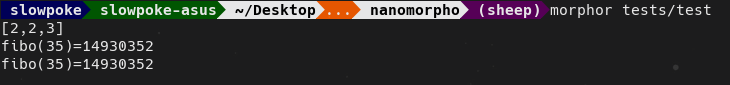
\includegraphics[width=0.8\textwidth]{test_nm_out.png}
  \end{figure}
\end{answer}

\end{document}
